\frame{
    \frametitle{Experiments metabolite identification}
    
\begin{block}{Dataset}
\begin{itemize}
    \item 342 reversed phase LC-retention times
    \item[$\circ$] for 120 MS/MS spectra available $\rightarrow$ (MS/MS, RT)-tuple
    \item[$\circ$] remaning 222 RTs are used for RankSVM training (\emph{target})
    \item 5 datasets (\emph{others}) of previous experiments also used for RankSVM training
\end{itemize}
\end{block}
\vspace{-0.25cm}   
\begin{block}{Evaluation measure and protocol}
\begin{itemize}
    \item randomly sample 1000 times 80 (MS/MS, RT)-tuples
    \item Construction of the graph containing the candidates to run the shortest path algorithm.
    \item Percentage of correct identifications for different values of $D$
    \item Comparison to baseline performance when $D=0$
\end{itemize}
\end{block}
}

\frame{ 
    \frametitle{Experiments metabolite identification}
    \framesubtitle{Baseline performance $22.7\%$: ($D=0$, only MS/MS spectra used, black line)}
    
\begin{figure}
    \centering
    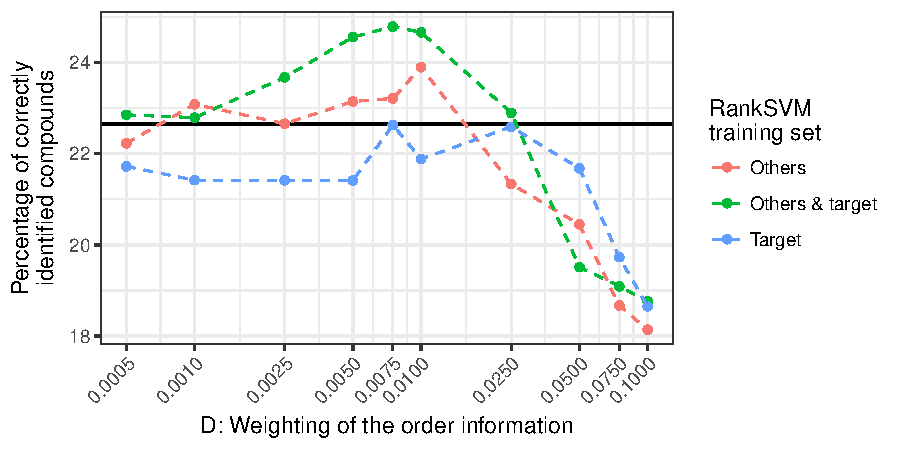
\includegraphics[width=0.9\textwidth]{images/top1_accuracy_reranking_GS_BS_n_rep_1000_no_facet.pdf}
\end{figure}
\vspace{-0.35cm}
\begin{small}
% \only<1>{
% \begin{table}
%     \centering
% \begin{tabular}{l|c|c}
%     \toprule
%     (only) Target & $\Pref(\sys_{Impact})$ & 222 RTs\\
%     (only) Others & $\bigcup_{\sys \in \hat{S}} \Pref(s)$ & 1098 RTs\\
%     Others \& target & $\bigcup_{\sys \in \hat{S}} \Pref(s) \cup \Pref(\sys_{Impact})$ & 1320 RTs\\
%     \bottomrule
% \end{tabular}
% \end{table}
% }
\only<1>{
\begin{block}{Observations}
\vspace{-0.15cm}
\begin{itemize}
    \item Improved identification accuracy for \emph{Others} ($23.9\%$) and \emph{Others \& target} ($24.8\%$)
    \item RankSVM trained only on the \emph{target} data cannot improve.
\end{itemize}
\end{block}
}
\end{small}
}
